\documentclass[12pt, letterpaper]{article}
\usepackage{bbold}
\usepackage{indentfirst}
\usepackage{amsmath, amssymb}
\usepackage[T1]{fontenc}
\usepackage[utf8]{inputenc}
\usepackage{physics}
\usepackage{tensor}
\usepackage{braket}
\usepackage{graphics}
\usepackage{grffile}
\usepackage[export]{adjustbox}
\usepackage{svg}
\usepackage{caption}
\usepackage{subcaption}
\usepackage{authblk} 
\usepackage{blindtext}
\usepackage{setspace}

\title{}

\begin{document}
    \section*{Report On Using MCMC Method To Find Hamiltonian And Thermalizaion of Berry-Keating And Damped Harmonic Oscillator}
    \subsection*{Preliminaries}
        Hamiltonian of Berry-Keating  
        \begin{equation}
            H = \frac{1}{2}(xp + px)
        \end{equation}
        \\
        
        and Damped Harmonic oscillator 
        \begin{equation}
            H = \frac{p^2}{2m} + \frac{1}{2}m \omega ^{2} x^{2} - \frac{p}{m} 
        \end{equation}

        We're using MCMC method to evaluate Hamiltonian and Thermalization of Berry-Keating and Damped harmonic oscillator. 
    
    \subsection*{Methodology}
        Markov Chain Monte Carlo (MCMC) is a random sampling method to visit x with a probability proportional to some given
        distribution say, $\pi (x)$. To use MCMC in simulation we first simplify the Hamiltonian Monte Carlo code in a block
        manner. Then we calculate and plot $<H>$ graphs of Berry-Keating and Damped harmonic oscillator Hamiltonian.
        
        \begin{adjustbox}{center,caption={Graph of Expectation value of Damped Harmonic Oscillator},nofloat=figure,label={somelabel}}
            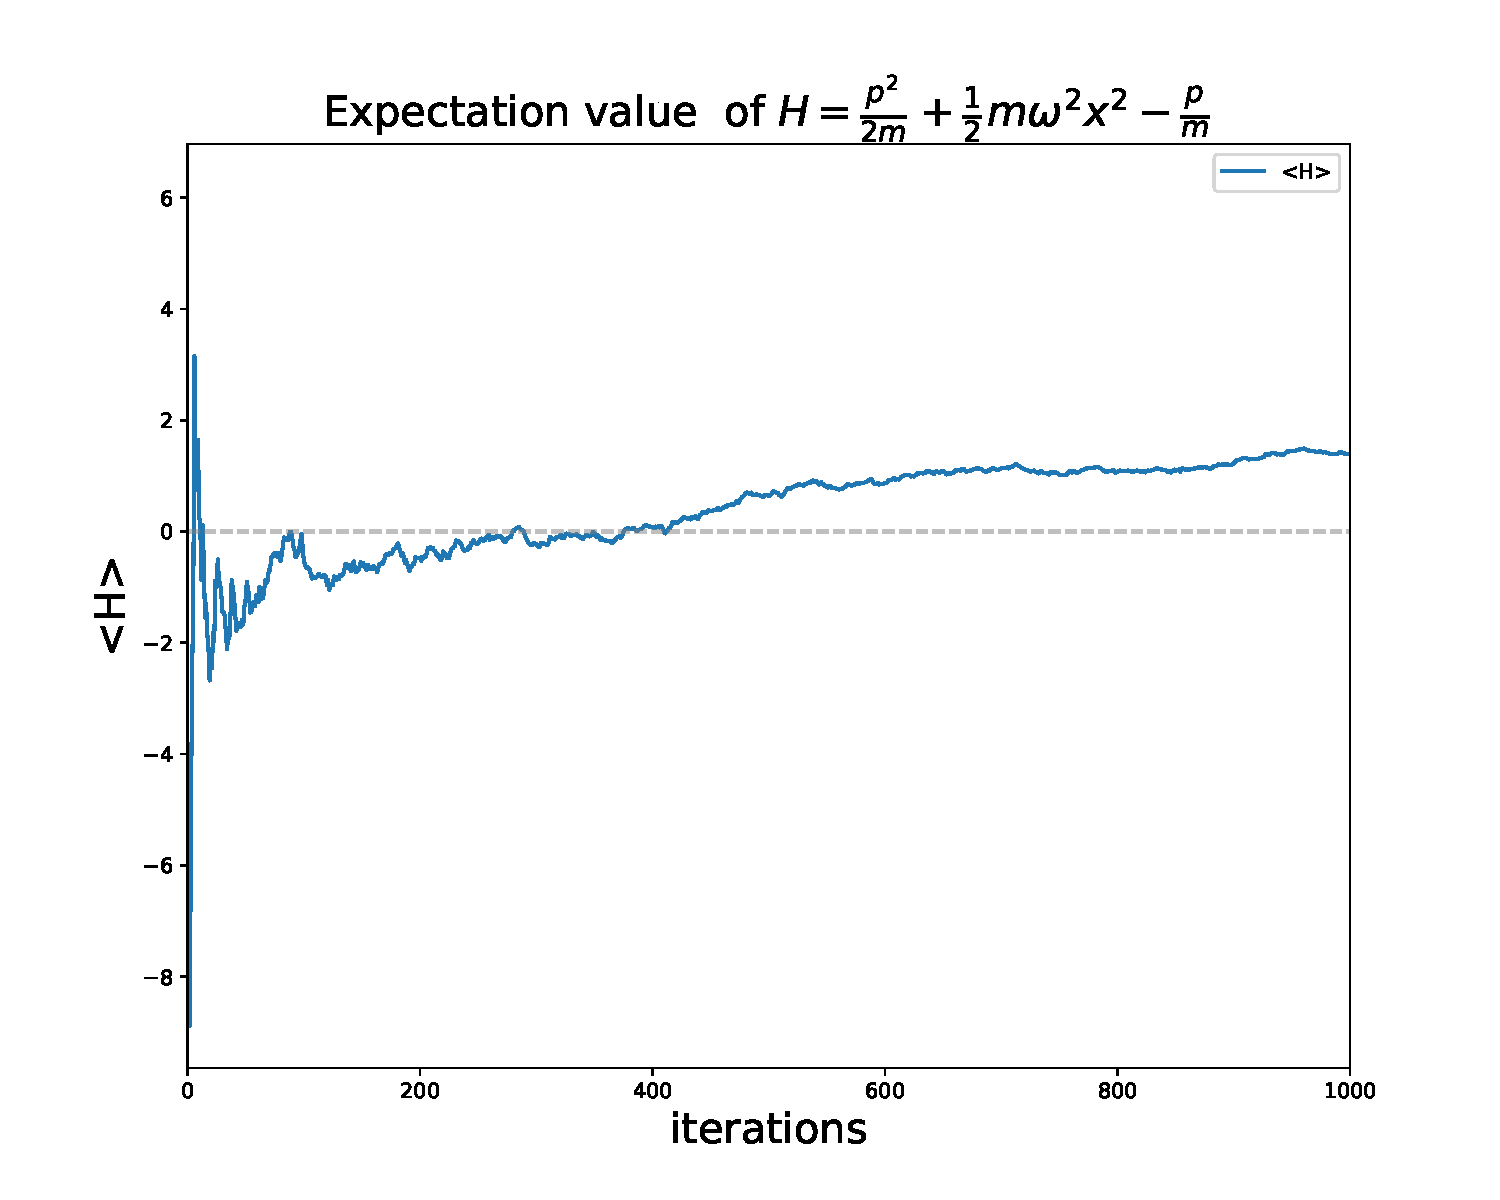
\includegraphics[width=0.8\textwidth]{dho.pdf}
        \end{adjustbox}

        \begin{adjustbox}{center,caption={Graph of Expectation value of Berry-Keating},nofloat=figure,label={somelabel}}
            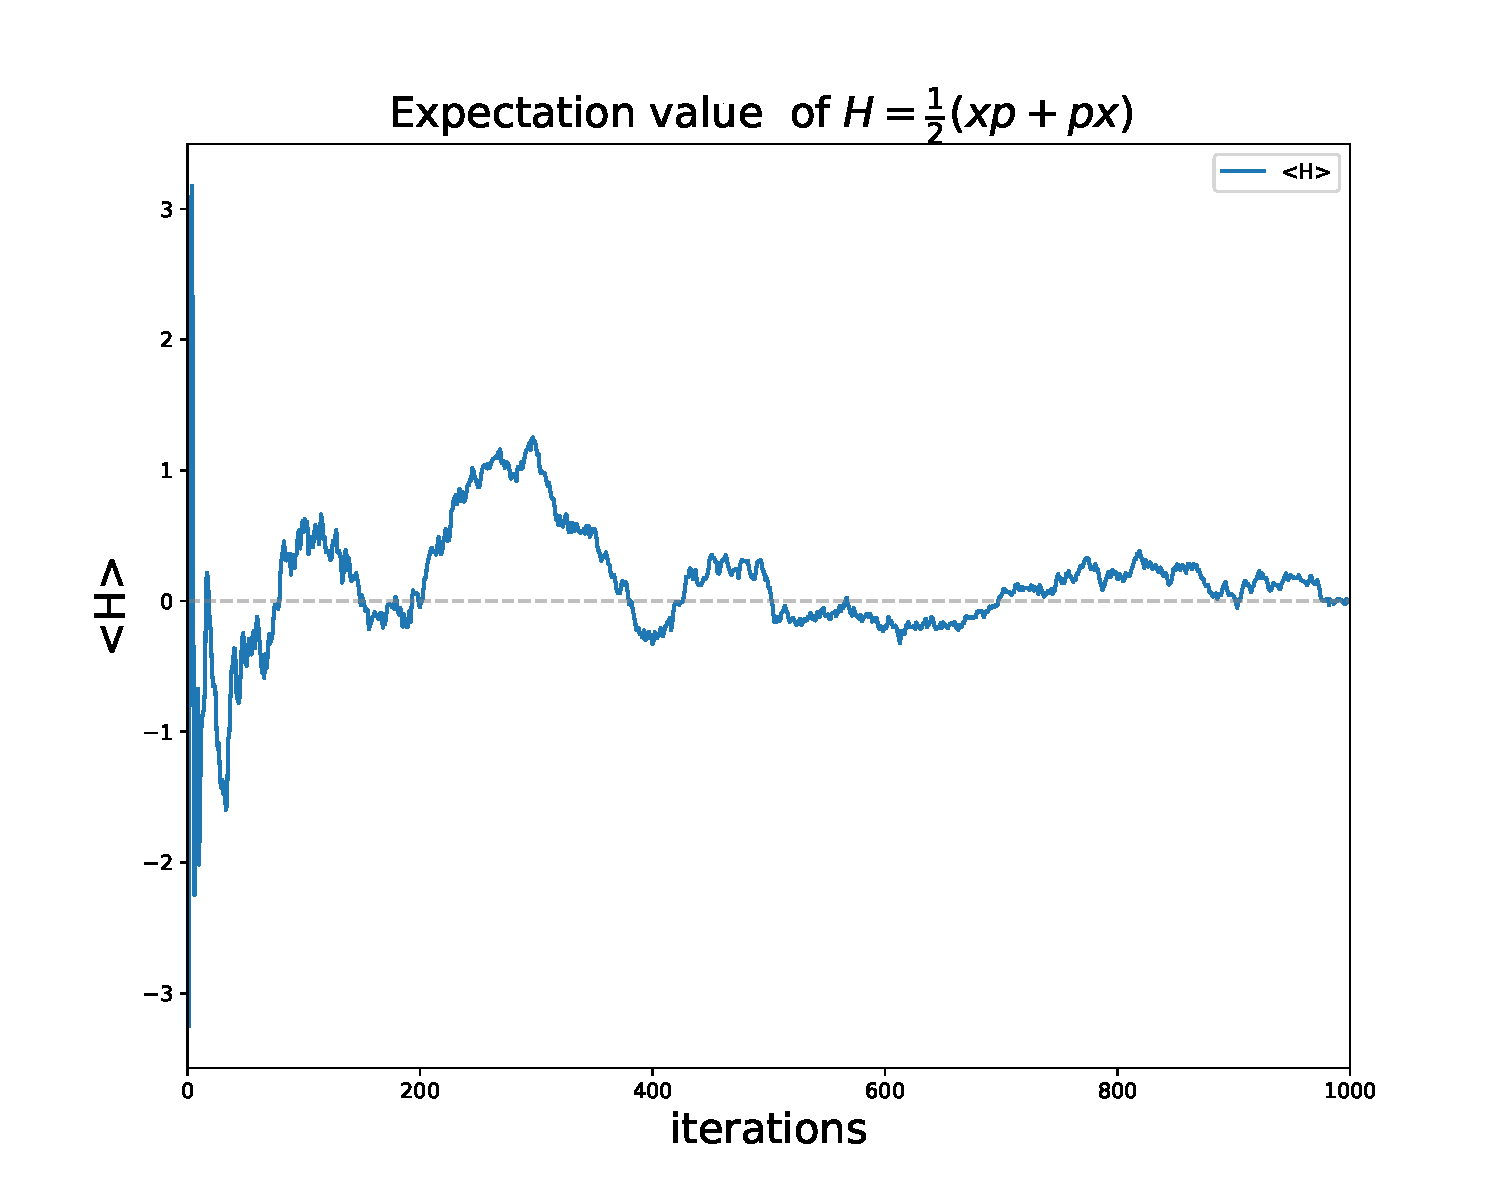
\includegraphics[width=0.8\textwidth]{bk.pdf}
        \end{adjustbox}
\end{document}